\begin{surferPage}[E6+- Singularity]{$E_6^{+-}$ Singularity}
	This singularity is given by the equation
	\[
		x^3+y^4-z^2=0.
	\]
	We cannot understand the geometry of this $E$ singularity by means of its picture, but we can deform it in two different ways: into two cusp singularities ($A_2$) or into one $D_5$ singularity. These can be seen by varying $a$ or $b$, respectively, in the equation
	\[
		x^2\cdot ((0.5-b)x-by)+y^2\cdot(y-a)^2-z^2.
	\]
	Keeping $b=0$ and varying $a$, we get:
	\begin{center}
		\begin{tabular}{c@{\quad}c@{\quad}c}
			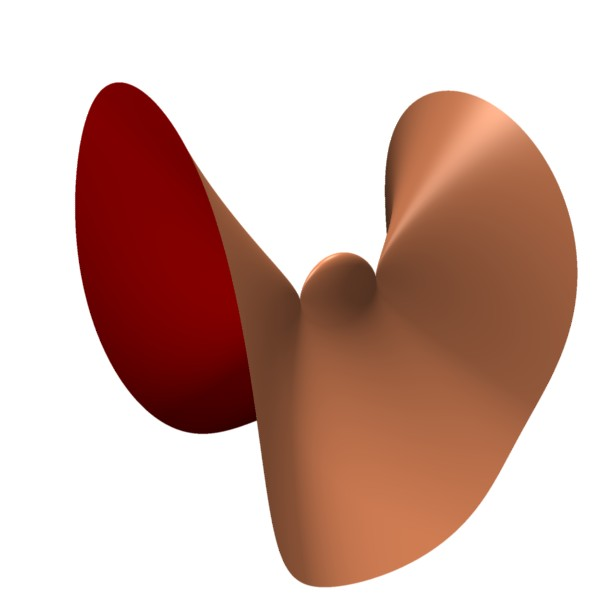
\includegraphics[width=1.1cm]{../../common/images/E6pm_1} &
			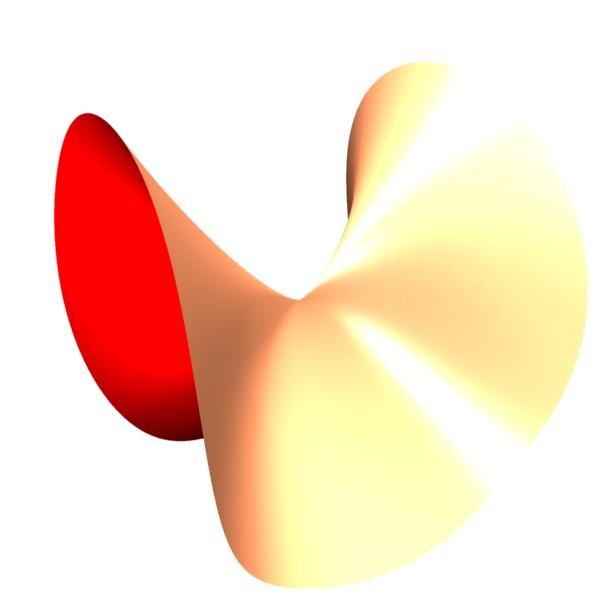
\includegraphics[width=1.1cm]{../../common/images/E6pm_0} &
			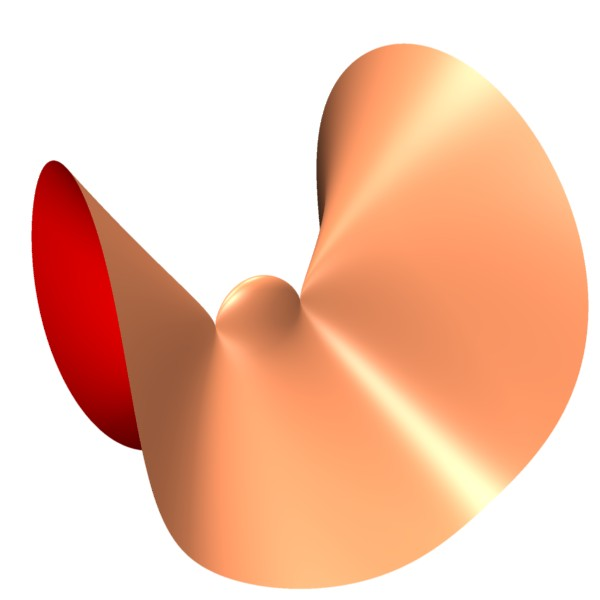
\includegraphics[width=1.1cm]{../../common/images/E6pm_2}\\
			$a=-0.5$ &
			$a=0$ &
			$a=0.5$
		\end{tabular}
	\end{center}
	On the other hand, keeping $a=0$ and varying $b$, yields:
	\begin{center}
		\begin{tabular}{c@{\quad}c@{\quad}c}
			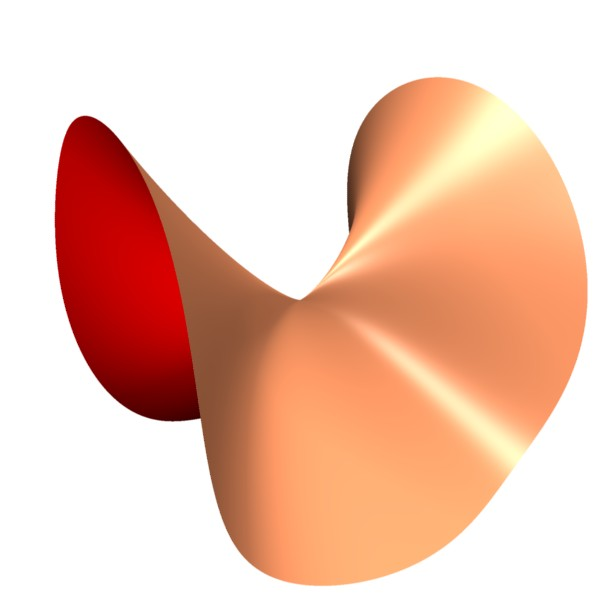
\includegraphics[width=1.1cm]{../../common/images/E6pm_4} &
			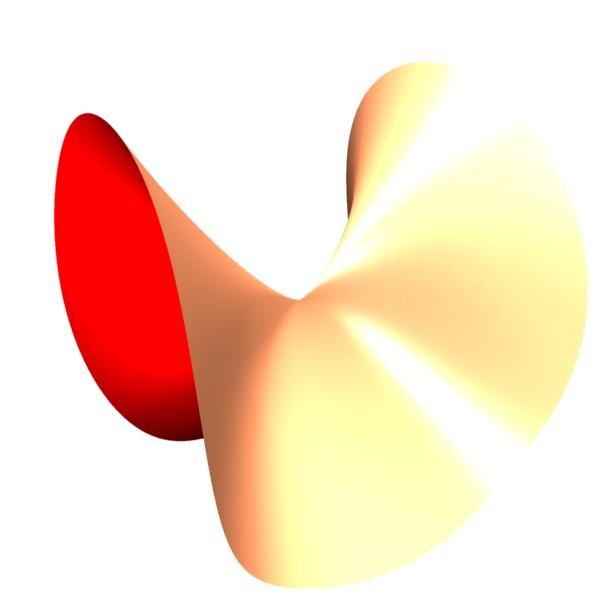
\includegraphics[width=1.1cm]{../../common/images/E6pm_0} &
			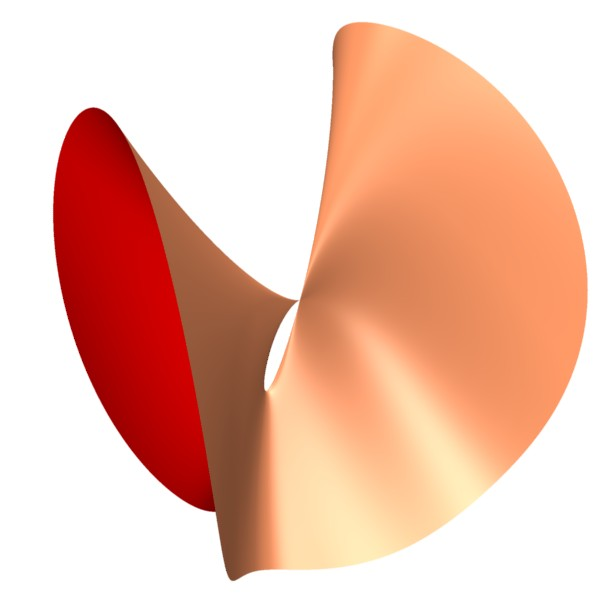
\includegraphics[width=1.1cm]{../../common/images/E6pm_5}\\
			$b=-0.5$ &
			$b=0$ &
			$b=0.5$
		\end{tabular}
	\end{center}
\end{surferPage}
